\documentclass[conference]{IEEEtran}
\IfFileExists{cite.sty}{\usepackage{cite}}{}
\usepackage{amsmath,amssymb}
\usepackage{graphicx}
\usepackage{booktabs}
\usepackage{array}
\renewcommand{\arraystretch}{1.12}
\usepackage{url}
\renewcommand{\ttdefault}{cmtt}
\newcommand{\pp}{\,\mathrm{pp}}
\newcommand{\method}[1]{\textsc{#1}}
\newcommand{\candb}{\textsc{Candidate B}}
\newcommand{\bdoc}{\textsc{B-Doc}}
\newcommand{\bshort}{\textsc{B-Short}}
\newcommand{\bhard}{\textsc{B-Hard}}
\newcommand{\af}[1]{\textsc{AF#1}}
\title{ContinualGuard: Continual Indirect Prompt-Injection Detection under Malicious and Benign Distribution Shift}
\author{\IEEEauthorblockN{Leshan Tang, Haoxiang Liao}
\IEEEauthorblockA{The University of Auckland, Auckland, New Zealand}}
\begin{document}
\maketitle
\begin{abstract}
Indirect prompt injection hides adversarial instructions in external content consumed by a language-model application. We study whether a binary detector retains earlier malicious patterns and accepts benign instruction-like text when updated sequentially. We build Candidate B, a prospectively frozen four-stage benchmark with matched document, short-form, and hard-benign arms, and evaluate a fixed DeBERTa-v3-base detector across three seeds. Current-only training loses $35.000\pm38.115$ percentage points of B-Short Stage-2 attack recall and raises B-Hard benign false-positive rate by $20.370\pm18.736$ points; both effects vary greatly by seed. Four bounded replay methods reduce these failures, while extra current-only training does not reproduce their endpoints. A controlled selector ablation fixes ranks, numerical settings, and buffer order: class and historical-stage quotas alter memory membership but show no consistent additional security gain. Coverage does not bind on the actual pools, and the proposed security-risk score is monotone-equivalent to true-label cross-entropy under a shared binary model state. Our evidence is restricted to this constructed offline benchmark; no independent malicious-stream confirmation or deployment test was completed.
\end{abstract}
\begin{IEEEkeywords}
indirect prompt injection, continual learning, experience replay, over-defense, benchmark evaluation
\end{IEEEkeywords}


\section{Introduction}
Retrieval-augmented and tool-integrated language-model applications process text from sources outside the user's control. Indirect prompt injection exploits this boundary by placing instructions in retrieved content rather than directly in the user's request \cite{greshake2023indirect}. Recent work formulates IPI defense as binary detection over external documents and studies both detection and removal under static conditions \cite{chen2025indirect}. A deployed detector, however, may be updated repeatedly as attack patterns and input distributions change. Each update can alter behavior on previously learned inputs.

Sequential updates create two security-relevant failure directions. A detector can forget earlier malicious patterns, increasing false negatives, or become over-defensive and reject benign text with instruction-like cues. PIGuard documents the latter behavior in static guard evaluation and introduces NotInject, a 339-record benign diagnostic bank \cite{li2025piguard}. CAPTURE also motivates context-sensitive attack and benign evaluation, but its malicious task is direct, single-turn prompt injection rather than IPI \cite{kholkar2025capture}. Neither evaluates staged continual adaptation of an IPI detector.

Continual learning separates plasticity, the acquisition of new behavior, from stability, the preservation of earlier behavior. Replay is a natural intervention: bounded historical examples are interleaved with current data to reduce interference \cite{rolnick2019experience,buzzega2020dark,buzzega2020rethinking}. We investigate three questions: \textbf{RQ1}, how evolving malicious and benign distributions affect attack retention, benign acceptance, and acquisition; \textbf{RQ2}, to what extent bounded replay mitigates these failures compared with current-only sequential and offline full-history training; and \textbf{RQ3}, whether increasingly structured replay-memory selectors consistently improve retention beyond simple balanced replay, and which component effects can be identified under controlled comparisons. All efficacy conclusions are conditional on the constructed \candb{} stream.

Our empirical contributions are fourfold. First, we evaluate malicious forgetting and benign over-defense during sequential IPI detection while separating acquisition from retention. Second, we construct \candb{}, a matched document/short-form/hard-benign benchmark that exposes failures hidden by simpler saturated streams. Third, we compare generic and structured replay with current-only and offline full-history controls under a fixed detector. Fourth, a controlled shared-rank, canonical-order A0-v2/A1/A2-canonical comparison tests class and historical-stage quotas separately; we audit a nonbinding coverage rule and show that the project risk score is monotone-equivalent to cross-entropy. We do not claim a new detector architecture or semantic scoring algorithm.

We expected a stream that changes both malicious and benign inputs to reveal two distinct failures: loss of earlier attack recall and increased benign rejection. We also tested whether historical replay would reduce both more than additional current-stage exposure, and whether structured selection would add value beyond simple replay. These expectations motivated the experiments; they were not preregistered hypotheses, and benchmark selection followed two earlier saturated pilots. The report therefore treats all effect estimates as conditional on Candidate B rather than evidence of deployment generality.

\section{Related Work}
\paragraph{Indirect prompt injection.}
IPI embeds adversarial instructions in externally supplied data that an application later retrieves or processes \cite{greshake2023indirect}. Chen et al. \cite{chen2025indirect} construct injected-document data and evaluate detection and removal with attack constructions including Ignore, Escape-Separation, Fake Completion, and Combined attacks. Their released artifacts provide our malicious-data and detector reference. Our data are a deterministic reconstruction from pinned artifacts, not an exact reproduction.

\paragraph{Over-defense.}
Prompt guards can rely on instruction-associated surface cues and flag benign text. PIGuard studies this problem and releases NotInject, whose benign examples contain common injection-related trigger words \cite{li2025piguard}. CAPTURE studies context-aware direct injection and benign behavior \cite{kholkar2025capture}. We use PIGuard to motivate hard-benign evaluation and NotInject only as a frozen diagnostic bank. CAPTURE informs safe-context design; no CAPTURE record is used or relabeled as malicious IPI.

\paragraph{Other agent data.}
WAInjectBench reports 991 malicious and 2,707 benign text segments from web-agent observations, including comments, messages, captions, and interface text \cite{liu2026wainjectbench}. These published counts are not a qualified sequential detector stream for our study: component usage terms, source-parent splits, overlap, and a prospective stage order remain unaudited. Likewise, public agent IPI test cases do not become binary detector records without defining a fixed observation and benign counterpart.

\paragraph{Continual replay.}
Experience replay preserves a bounded sample of the past \cite{rolnick2019experience,buzzega2020rethinking}. Dark Experience Replay stores historical logits; DER++ additionally uses replay labels \cite{buzzega2020dark}. Gradient-based sample selection (GSS) emphasizes memory diversity in gradient space \cite{aljundi2019gradient}, while maximal interfered retrieval (MIR) chooses replay items whose predictions are expected to deteriorate under an update \cite{aljundi2019mir}. These are relevant selection mechanisms, not methods reproduced here. Poor current-stage learning and forgetting are distinct, so acquisition must be checked before interpreting later score changes \cite{elsayed2024plasticity}. These established replay studies motivate controlled mechanisms in the fixed-label IPI setting; we do not assert that prior security work lacked possible remedies.

\section{Methodology}
\subsection{Task and evaluation measures}
Stages arrive in order \af{2}$\rightarrow$\af{3}$\rightarrow$\af{4}$\rightarrow$\af{5}. At stage $t$, a binary detector $f_\theta(x)$ learns current-stage examples with label 0 for benign content and label 1 for IPI. Model weights carry forward; AdamW state is reset. After each stage, the detector is evaluated on every seen test stage. The research code and aggregate results are publicly available.\footnote{\url{https://github.com/Ukino13t/ContinualGuard}}

Acquisition is performance immediately after learning a stage. For a higher-is-better metric $m$, final backward transfer over the $T-1$ earlier stages is
\begin{equation}
\mathrm{BWT}_m=\frac{1}{T-1}\sum_{i=1}^{T-1}\left(m_{T,i}-m_{i,i}\right).
\end{equation}
For each earlier stage we calculate the largest nonnegative attack-TPR decline from its best checkpoint so far, then average those stagewise maxima to obtain the run-level peak-forgetting summary. For benign false-positive rate (FPR), we report the mean signed final-minus-acquisition change across earlier stages, so positive values are harmful. Attack true-positive rate (TPR), benign FPR, macro-F1, and accuracy remain separate: high attack recall cannot compensate for rejecting benign inputs.
Worst-group diagnostics take the maximum acquisition-to-final FPR increase over available benign metadata groups and the maximum attack-TPR decrease over head, middle, and tail positions of earlier stages, flooring both at zero. They are descriptive maxima over the pre-existing groups, not independently estimated population risks. Each position slice has 20 malicious test items, hence 5-pp resolution.

Replay entry follows a prospective three-state policy. R0 means replay is not justified; R1 records limited evidence; R2 requires a predeclared harmful magnitude, cross-seed directional consistency, and matched evidence. These states decide whether replay may be studied, not which replay method wins.
\subsection{Benchmark selection and stage design}

The first family-disjoint stream used Naive, Ignore, Escape-Separation, and Fake Completion. Acquisition approached the ceiling and retention changes were small or transient. H2-mini then introduced independently reviewed benign pressure, but its control and hard-benign arms both had attack-TPR BWT of zero. Replay remained blocked at R0. \candb{} was the final escalation. Its No Replay result reached R2, after which benchmark development stopped and replay methods were frozen.

\subsection{Human-reviewed benign data}

Two independent reviewers applied a fixed rubric covering benign eligibility, ambiguous or unsafe intent, missing context, privacy and rights concerns, and true injection. A 50-record calibration achieved 96\% exact decision agreement and zero benign-versus-true-injection conflicts. Production review revealed severe disagreement over proposed B1/B2/B3 difficulty strata, so the taxonomy was simplified prospectively to ordinary benign (B0) and source-defined hard benign (BH). BH-1/BH-2/BH-3 are balanced disjoint partitions, not ordinal difficulty levels. Validation and test records required independent double acceptance; acceptance conflicts were excluded. Production review yielded 2,288 judgments over 1,590 candidates: 95.85\% exact decision agreement but only 45.70\% stratum agreement. The simplified B0/BH taxonomy avoids treating disputed strata as ground truth. Validation and test records required two independent acceptances; exact, normalized, model-view, substring, lexical, semantic-neighbor, and template overlap checks were performed. One semantic-neighbor B0 record was quarantined. These checks reduce known overlap without proving universal semantic independence.

\subsection{Candidate B}

\candb{} contains three four-stage arms (Table~\ref{tab:benchmark}). Every arm-stage has 400 train, 60 validation, and 120 test examples, balanced by label; each test set therefore has 60 malicious and 60 benign examples. Arms share malicious identifiers, splits, families, and head/middle/tail injection positions. All arms share the first-stage document anchor, and \bshort{} and \bhard{} remain identical through Stage 2. The sequence is Ignore, Escape-Separation, Fake Completion, and Combined. \af{5} is compositional and is not treated as a family-disjoint unseen attack.

\begin{table}[t]
\caption{The three matched \candb{} arms. Each arm-stage contains 400/60/120 train/validation/test records with 50/50 labels.}
\label{tab:benchmark}

\centering
\small
\setlength{\tabcolsep}{5pt}
\begin{tabular}{@{}lll@{}}
\toprule
Arm & Benign context after anchor & Malicious stages \\
\midrule
\bdoc & document controls & \af{2}--\af{5} \\
\bshort & ordinary short-form & \af{2}--\af{5} \\
\bhard & reviewed hard benign & \af{2}--\af{5} \\
\bottomrule
\end{tabular}


\end{table}

\begin{table*}[t]
\caption{Frozen \candb{} stage composition.}
\label{tab:stage-composition}

\centering
\small
\setlength{\tabcolsep}{5pt}
\begin{tabular}{@{}llllll@{}}
\toprule
Stage & Malicious family & \bdoc{} benign & \bshort{} benign & \bhard{} benign & Train / val / test per arm \\
\midrule
\af{2} & Ignore & D0-1 & D0-1 & D0-1 & 400 / 60 / 120 \\
\af{3} & Escape-Separation & D0-2 & B0-2 & B0-2 & 400 / 60 / 120 \\
\af{4} & Fake Completion & D0-3 & B0-3 & BH-1 & 400 / 60 / 120 \\
\af{5} & Combined (compositional) & D0-4 & B0-4 & BH-2 & 400 / 60 / 120 \\
\bottomrule
\end{tabular}


\end{table*}

Matched anchors improve interpretation but do not isolate a single causal factor. Source, language, length, format, and semantics remain bundled across arms. The benign test resolution is $1/60=1.667\pp$, as is the malicious TPR resolution.

\begin{table}[t]
\caption{Human-review calibration before production review.}
\label{tab:calibration}

\centering
\small
\begin{tabular}{@{}lr@{}}
\toprule
Calibration statistic & Value \\
\midrule
Records / judgments & 50 / 100 \\
Exact decision agreement & 48/50 (96.00\%) \\
Decision Cohen's $\kappa$ & 0.8255 \\
Stratum agreement & 47/50 (94.00\%) \\
Stratum Cohen's $\kappa$ & 0.7956 \\
Binary benign agreement & 49/50 (98.00\%) \\
Benign vs. true-injection conflicts & 0 \\
Mean / median review time & 19.26 / 20.00 s \\
\bottomrule
\end{tabular}


\end{table}
\subsection{Learning methods and controls}
\paragraph{No Replay (M0).}
The model trains only on the current stage.

\paragraph{Reservoir ER (M1).}
A standard unstratified online reservoir stores 200 historical training examples and is sampled uniformly. One replay batch accompanies every current-data minibatch once memory is nonempty.

\paragraph{DER++ (M2).}
DER++ uses the same reservoir identities and stores two historical logits per example \cite{buzzega2020dark}. The loss combines current cross-entropy (CE), replay-label CE, and replay-logit mean squared error with $\alpha=\beta=0.5$. We divide their sum by $1+\alpha+\beta$ to control loss scale; this normalization is a project choice.

\paragraph{Security-aware Replay (M3).}
The 200-example memory contains exactly 100 benign and 100 malicious records. Deterministic historical-stage quotas are filled after preferring one example per available coverage key; hashes break ties. Before each stage update, candidates from training data are scored once using
\begin{equation}
r(x,y)=
\begin{cases}
1-p_{\mathrm{attack}}(x), & y=1,\\
p_{\mathrm{attack}}(x), & y=0.
\end{cases}
\end{equation}
The training loss matches Reservoir ER: $(L_{\mathrm{current}}+L_{\mathrm{replay}})/2$. Validation, test, external banks, and future stages never enter selection.

\paragraph{Generic Loss-aware Replay (M4).}
This matched control fixes the M3 capacity, exposure, class/stage quotas, coverage rule, replay loss, and deterministic ties, changing only the frozen pre-update score to true-label CE, $d(x,y)$. Under a common binary model state,
\begin{equation}
d(x,y)=-\log\bigl(1-r(x,y)\bigr),
\end{equation}
which is strictly monotone. Operational differences begin with finite-precision scores and ties and compound after memory choices create different model trajectories. M4 tests selector behavior without attributing it to uniquely security-specific score semantics.

\paragraph{Memory-structure ablation (A0--A5).}
Historical A0 reuses M1 online Reservoir and A5 reuses M3 Security-aware. A1 retains 100 examples of each label by hash rank; A2 additionally divides each label quota over historical stages. A3 prefers one record per coverage key before residual filling, and A4 uses the true-label CE score under A3 constraints. The original A1--A3 sequence used variant-specific hashes. The later matched A1/A2 pair shared ranks but stored selected items in different orders, changing index-based replay identities even when membership agreed. Our controlled comparison uses A0-v2 (global bottom-$M$ ranks), A1 (class quotas), and A2-canonical (class and stage quotas). All three store selected items in the same (label, rank, ID) order and use the same eligible pool rule $B_{t-1}\cup D_t^{\mathrm{train}}$. For each of the nine A1/A2-canonical pairs, initialization, current-example order, replay policy, AMP initial scale 256, training budget, and all other effective settings match; the first two stages also reproduce exact training logs and model hashes. A2-canonical retains the historical matched A2 selected-ID set, but corrects its buffer order. Historical matched A2 outcomes remain provenance, not an isolated stage-quota effect. Original Reservoir, A4, and A5 are contextual controls under the earlier numerical protocol.

In all 36 actual arm--seed--stage eligible pools, every coverage key is unique. Under the shared rank, A2 and A3 select the same ordered memory at every update; a two-stage independent training check gives identical weights, training logs, and buffers. Thus a full A3 rerun would duplicate A2 and cannot estimate a coverage effect. The original A3 trajectories remain in the historical record but are not treated as evidence for coverage.

\paragraph{Bounded-memory update.}
For M3/M4, let $B_{t-1}$ be the retained buffer and $D_t^{\mathrm{train}}$ the newly arrived training stage. The eligible update pool is $B_{t-1}\cup D_t^{\mathrm{train}}$; discarded historical examples are not reintroduced. The incoming model scores only $D_t^{\mathrm{train}}$ before adaptation. After current-stage training, the selector allocates 100 slots per label, divides each label's quota among contributed stages with earlier-stage remainder, sorts eligible examples by the frozen score and deterministic hash, takes one example per coverage key when possible, and fills residual quota in score order. During stage $t$, each current minibatch uses up to four uniformly sampled records from $B_{t-1}$; $D_t^{\mathrm{train}}$ becomes replay-eligible only at stage $t+1$. The local implementation reconstructs stored text by retained ID from local TRAIN files, a data-access assumption distinct from the bounded set of selected replay identities. No raw prompt text appears in memory audit summaries.

\paragraph{Exact selector procedure.}
At stage $t$, the incoming model scores every member of $D_t^{\mathrm{train}}$ once before any optimizer update and retains each older memory item's frozen score. The model then trains on the current stage, sampling up to four uniformly drawn records from $B_{t-1}$ alongside each current four-record minibatch. The next eligible pool is exactly $C_t=B_{t-1}\cup D_t^{\mathrm{train}}$; an item discarded at an earlier stage cannot return. In each label, the structured selector allocates 100 slots across represented historical stages, assigning remainders to earlier stages. It ranks eligible records by frozen score and a deterministic SHA-256 tie key, selects at most one from each coverage key when possible, and fills residual slots by rank. The selected IDs, order, metadata, and buffer RNG are serialized. This procedure never accesses future, validation, test, or external diagnostic records. Reservoir instead uses standard online replacement over current training examples; DER++ records two logits with each stored item.

\paragraph{Matched intervention.}
Original A1--A3 selectors used variant-specific hash namespaces, so their adjacent differences confound rank and quota. A later A1/A2 comparison shared ranks but changed replay-buffer order; index-based uniform replay can then expose different records. We use the corrected A0-v2/A1/A2-canonical comparison, holding rank, buffer order, AMP initial scale 256, optimizer, capacity, replay policy, and current-example sequence fixed. A0-v2 imposes no label quota, A1 adds a 100/100 label quota, and A2-canonical additionally allocates quotas by historical stage. Actual coverage keys are unique in all 36 arm--seed--stage pools: shared-rank A2 and A3 therefore select identical ordered memory and cannot estimate a coverage effect. A separate two-stage parity test confirmed identical weights and logs.
\subsection{Experimental protocol and reproducibility}
All methods use \texttt{microsoft/deberta-v3-base}, revision \texttt{8ccc9b6f...53f3}, maximum length 1280, seeds 17/42/2026, one epoch per stage, batch size 4, AdamW at $10^{-5}$, constant scheduling, FP16 CUDA, optimizer reset, and carried weights. Prediction uses binary-logit argmax, equivalent to $p_{\mathrm{attack}}=0.5$ with ties assigned benign. Replay methods use capacity $M=200$ and replay batch size 4.

We report means and sample SD across three fixed seeds without significance claims. The one-epoch joint reference performs 400 updates over 1,600 TRAIN records. Current-only processes two shuffled current minibatches per update over 100 updates per stage, without historical training examples.

Every arm-stage contains 200 positive and 200 negative training examples, 30 of each in validation, and 60 of each in test. The full four-stage arm therefore contains 1,600 training examples and 480 test examples; the 15 primary method--arm combinations at three seeds yield 45 runs and 180 stage-end checkpoints. We calculate accuracy, macro-F1, attack TPR, and benign FPR from raw predictions on each previously seen frozen test set. Current-stage acquisition is measured immediately after its training update. We report sample standard deviations rather than confidence intervals because the fixed three seeds are insufficient for a strong population inference. Each class-conditional stage-test rate changes in steps of $1/60=1.667\pp$, and each 20-example attack-position slice in 5\,pp. No test result is used to select memory or tune a threshold.

The training environment was Python 3.14.5, PyTorch 2.14.0+cu126, Transformers 4.57.6, CUDA 12.6, and an NVIDIA GeForce RTX 2060. Complete primary-run time ranged from 3.56 minutes for No Replay to 6.45 minutes for Loss-aware; peak allocated GPU memory was about 3.53\,GiB. The repository retained configuration hashes, checkpoint lineage, stage-level predictions, and memory selected IDs. Raw prompt text and reviewer notes are not distributed with this report.

\section{Implementation and Results}
\subsection{Sequential failure and replay mitigation}

Table~\ref{tab:primary} gives the frozen primary comparison. Negative attack ``loss'' denotes positive backward transfer; negative FPR increase means the final FPR is lower than at acquisition.

\begin{table*}[t]
\caption{Primary results across three seeds (mean $\pm$ sample SD).}
\label{tab:primary}

\centering
\small
\setlength{\tabcolsep}{4.4pt}
\begin{tabular}{@{}lrrrr@{}}
\toprule
Method & \bshort{} \af{3} TPR loss & \bhard{} FPR increase & \bhard{} D0-1 FPR change & Acquisition \\
& (pp) & (pp) & (pp) & gates \\
\midrule
No Replay & 35.000 $\pm$ 38.115 & 20.370 $\pm$ 18.736 & 62.222 $\pm$ 54.297 & 12/12 \\
Reservoir ER & -0.556 $\pm$ 2.546 & 1.481 $\pm$ 3.060 & 5.000 $\pm$ 8.660 & 12/12 \\
DER++ & 0.000 $\pm$ 1.667 & 0.370 $\pm$ 1.156 & 1.667 $\pm$ 2.887 & 12/12 \\
Security-aware & 1.111 $\pm$ 0.962 & -0.556 $\pm$ 0.962 & 0.000 $\pm$ 0.000 & 12/12 \\
Loss-aware & -0.556 $\pm$ 0.962 & 0.185 $\pm$ 0.321 & 1.111 $\pm$ 1.925 & 12/12 \\
\bottomrule
\end{tabular}


\end{table*}

No Replay loses $35.000\pm38.115\pp$ of \bshort{} \af{3} attack TPR from acquisition to the final \af{5} checkpoint. Seed losses are 20.000, 6.667, and 78.333 pp: the magnitude is unstable, but the direction is harmful in all three seeds. Reservoir ER, DER++, Security-aware, and Loss-aware reduce the mean loss to $-0.556$, $0.000$, $1.111$, and $-0.556\pp$, respectively. Figure~\ref{fig:af3} shows the trajectory. Security-aware is not the strongest method on this endpoint.

\begin{figure}[t]
\centering
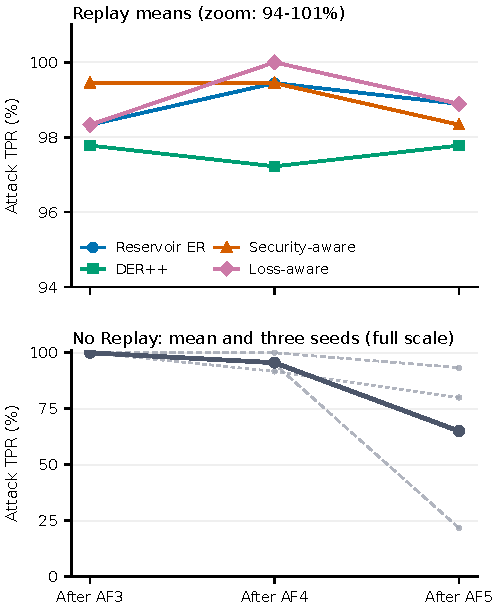
\includegraphics[width=\columnwidth]{figures/b_short_af3_retention.pdf}
\caption{\bshort{} \af{3} attack TPR after acquisition and later stages. The upper panel expands 94--101\% to distinguish replay-method means; the lower panel retains the full 0--100\% scale for the No Replay mean and all three seed trajectories. Different vertical scales are explicit.}
\label{fig:af3}
\end{figure}

The benign endpoint tells a complementary story. No Replay increases overall \bhard{} FPR by $20.370\pm18.736\pp$. The replay values are $1.481$, $0.370$, $-0.556$, and $0.185\pp$. On the shared D0-1 partition, No Replay changes by 0, 100, and 86.667 pp across seeds. Security-aware remains 0/0/0; Loss-aware is 3.333/0/0; Reservoir is 0/15/0; and DER++ is 0/0/5 pp. Security-aware has the lowest observed D0-1 FPR change in these three seeds; this sparse endpoint does not establish general dominance.

\begin{figure*}[t]
\centering
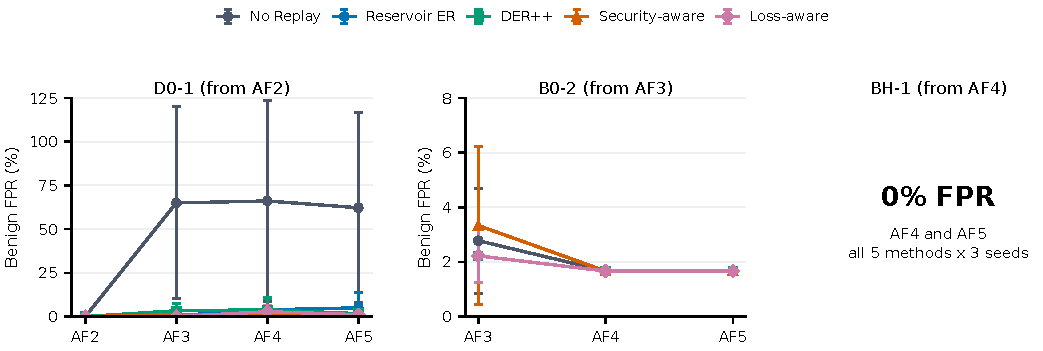
\includegraphics[width=0.97\textwidth]{figures/b_hard_benign_retention.pdf}
\caption{\bhard{} benign FPR trajectories (mean $\pm$ sample SD over three seeds). D0-1 and B0-2 use separately labeled vertical ranges of 0--125\% and 0--8\% so both partitions remain readable; the SD whisker is descriptive and can extend above a feasible individual FPR of 100\%. Every BH-1 observation is exactly zero at both checkpoints, so the third panel states the result instead of plotting coincident curves.}
\label{fig:benign}
\end{figure*}

\begin{figure*}[t]
\centering
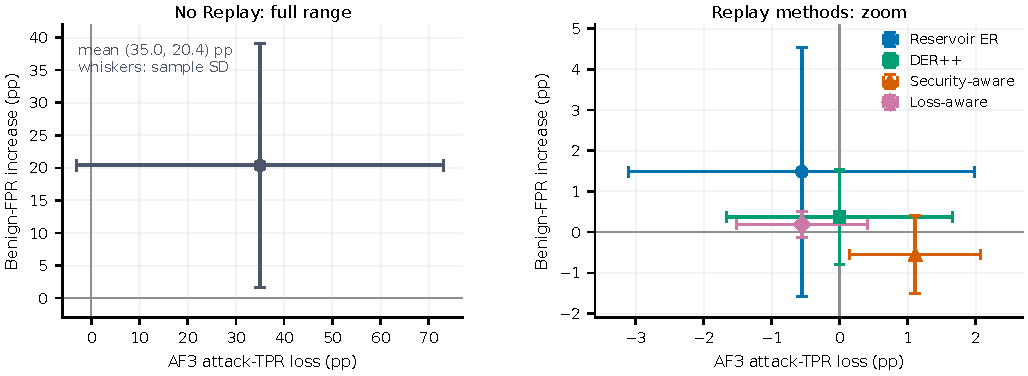
\includegraphics[width=0.90\textwidth]{figures/malicious_benign_tradeoff.pdf}
\caption{Mean \bshort{} \af{3} attack-TPR loss versus \bhard{} benign-FPR increase with sample-SD bars (percentage points; lower is better on both axes). The left panel shows No Replay on its full range; the separately scaled right panel resolves the four replay methods near the origin. These are descriptive run-to-run SDs, not confidence intervals.}
\label{fig:tradeoff}
\end{figure*}

\subsection{Full retention profile and seed variation}
The arm-level backward-transfer profile (Table~\ref{tab:arm-retention}) separates attack recall, macro-F1, benign-FPR increase, and peak attack forgetting. In B-Hard, No Replay's attack TPR remains nearly stable while macro-F1 drops: benign over-defense, rather than attack forgetting, is the dominant error. B-Short shows the opposite large attack-retention problem. The seed tables expose the discrete test outcomes behind these means.

\begin{table*}[t]
\caption{Arm-level retention summary (mean $\pm$ sample SD, pp).}
\label{tab:arm-retention}

\centering
\scriptsize
\setlength{\tabcolsep}{3.8pt}
\begin{tabular}{@{}llrrrr@{}}
\toprule
Method & Arm & Attack-TPR BWT & Macro-F1 BWT & Benign-FPR increase & Attack peak forgetting \\
\midrule
No Replay & B-DOC & -1.296 $\pm$ 0.849 & -0.648 $\pm$ 0.425 & 0.000 $\pm$ 0.000 & 1.481 $\pm$ 0.642 \\
No Replay & B-SHORT & -12.593 $\pm$ 13.256 & -12.184 $\pm$ 8.169 & 8.519 $\pm$ 16.200 & 12.778 $\pm$ 13.064 \\
No Replay & B-HARD & -0.185 $\pm$ 0.849 & -13.243 $\pm$ 11.656 & 20.370 $\pm$ 18.736 & 0.556 $\pm$ 0.962 \\
Reservoir ER & B-DOC & 0.370 $\pm$ 0.642 & 0.185 $\pm$ 0.321 & 0.000 $\pm$ 0.000 & 0.000 $\pm$ 0.000 \\
Reservoir ER & B-SHORT & 0.370 $\pm$ 1.156 & 0.278 $\pm$ 0.556 & -0.185 $\pm$ 0.321 & 0.185 $\pm$ 0.321 \\
Reservoir ER & B-HARD & 0.185 $\pm$ 1.398 & -0.653 $\pm$ 0.983 & 1.481 $\pm$ 3.060 & 0.370 $\pm$ 0.642 \\
DER++ & B-DOC & -0.741 $\pm$ 0.642 & -0.370 $\pm$ 0.321 & 0.000 $\pm$ 0.000 & 0.926 $\pm$ 0.849 \\
DER++ & B-SHORT & 0.370 $\pm$ 0.642 & 0.185 $\pm$ 0.161 & 0.000 $\pm$ 0.556 & 0.370 $\pm$ 0.321 \\
DER++ & B-HARD & -0.185 $\pm$ 1.697 & -0.278 $\pm$ 0.481 & 0.370 $\pm$ 1.156 & 1.296 $\pm$ 0.849 \\
Security-aware & B-DOC & 0.185 $\pm$ 0.321 & 0.093 $\pm$ 0.160 & 0.000 $\pm$ 0.000 & 0.000 $\pm$ 0.000 \\
Security-aware & B-SHORT & -0.556 $\pm$ 1.111 & -0.557 $\pm$ 1.004 & 0.556 $\pm$ 2.546 & 0.926 $\pm$ 1.156 \\
Security-aware & B-HARD & -0.556 $\pm$ 1.111 & 0.000 $\pm$ 0.278 & -0.556 $\pm$ 0.962 & 0.926 $\pm$ 0.849 \\
Loss-aware & B-DOC & 0.000 $\pm$ 0.556 & 0.093 $\pm$ 0.424 & -0.185 $\pm$ 0.321 & 0.185 $\pm$ 0.321 \\
Loss-aware & B-SHORT & 0.370 $\pm$ 0.321 & -0.465 $\pm$ 1.056 & 1.296 $\pm$ 2.245 & 0.370 $\pm$ 0.642 \\
Loss-aware & B-HARD & 0.741 $\pm$ 0.849 & 0.278 $\pm$ 0.556 & 0.185 $\pm$ 0.321 & 0.000 $\pm$ 0.000 \\
\bottomrule
\end{tabular}


\end{table*}

\begin{table}[t]
\caption{Per-seed \bshort{} \af{3} retention from acquisition to the final \af{5} checkpoint (percent or percentage points).}
\label{tab:af3-seed}

\centering
\scriptsize
\setlength{\tabcolsep}{3.4pt}
\begin{tabular}{@{}lrrrrr@{}}
\toprule
Method & Seed & Acq. TPR & Final TPR & TPR loss & F1 loss \\
\midrule
No Replay & 17 & 100.000 & 80.000 & 20.000 & 8.424 \\
No Replay & 42 & 100.000 & 93.333 & 6.667 & 3.336 \\
No Replay & 2026 & 100.000 & 21.667 & 78.333 & 45.430 \\
Reservoir ER & 17 & 100.000 & 100.000 & 0.000 & -0.834 \\
Reservoir ER & 42 & 96.667 & 100.000 & -3.333 & -1.667 \\
Reservoir ER & 2026 & 98.333 & 96.667 & 1.667 & 0.834 \\
DER++ & 17 & 100.000 & 100.000 & 0.000 & -0.834 \\
DER++ & 42 & 100.000 & 98.333 & 1.667 & 0.833 \\
DER++ & 2026 & 93.333 & 95.000 & -1.667 & -0.835 \\
Security-aware & 17 & 100.000 & 98.333 & 1.667 & -1.670 \\
Security-aware & 42 & 100.000 & 100.000 & 0.000 & 0.000 \\
Security-aware & 2026 & 98.333 & 96.667 & 1.667 & 0.834 \\
Loss-aware & 17 & 100.000 & 100.000 & 0.000 & -0.834 \\
Loss-aware & 42 & 100.000 & 100.000 & 0.000 & 0.000 \\
Loss-aware & 2026 & 95.000 & 96.667 & -1.667 & -0.834 \\
\bottomrule
\end{tabular}


\end{table}

\begin{table}[t]
\caption{Per-seed \bhard{} D0-1 benign FPR at acquisition and after \af{5}.}
\label{tab:d01-seed}

\centering
\scriptsize
\setlength{\tabcolsep}{4pt}
\begin{tabular}{@{}lrrrr@{}}
\toprule
Method & Seed & Acq. FPR & Final FPR & Change \\
\midrule
No Replay & 17 & 0.000 & 0.000 & 0.000 \\
No Replay & 42 & 0.000 & 100.000 & 100.000 \\
No Replay & 2026 & 0.000 & 86.667 & 86.667 \\
Reservoir ER & 17 & 0.000 & 0.000 & 0.000 \\
Reservoir ER & 42 & 0.000 & 15.000 & 15.000 \\
Reservoir ER & 2026 & 0.000 & 0.000 & 0.000 \\
DER++ & 17 & 0.000 & 0.000 & 0.000 \\
DER++ & 42 & 0.000 & 0.000 & 0.000 \\
DER++ & 2026 & 0.000 & 5.000 & 5.000 \\
Security-aware & 17 & 0.000 & 0.000 & 0.000 \\
Security-aware & 42 & 0.000 & 0.000 & 0.000 \\
Security-aware & 2026 & 0.000 & 0.000 & 0.000 \\
Loss-aware & 17 & 0.000 & 3.333 & 3.333 \\
Loss-aware & 42 & 0.000 & 0.000 & 0.000 \\
Loss-aware & 2026 & 0.000 & 0.000 & 0.000 \\
\bottomrule
\end{tabular}


\end{table}

\subsection{Offline and optimization controls}

The one-epoch joint reference sees all 1,600 legitimate TRAIN records at once and performs 400 updates. Across three seeds, its final mean attack TPR / benign FPR / macro-F1 across the four stage tests is $100.00/0.00/100.00\%$ in \bdoc{}, $99.58/0.83/99.37\%$ in \bshort{}, and $99.31/0.56/99.37\%$ in \bhard{}. This full-history result is strong and close to replay on the main endpoints, but a single epoch is a finite-optimization reference rather than an upper bound.

Across three seeds, two current-only minibatches per update improve \bshort{} final four-test attack TPR from $90.42\pm9.80\%$ to $93.61\pm5.69\%$, but Reservoir reaches $99.72\pm0.48\%$ under historical access (Table~\ref{tab:r2-compute}). Current-only \bshort{} TPR backward transfer remains negative ($-8.33\pm7.72\pp$), compared with Reservoir's $+0.37\pm1.16\pp$. In \bhard{}, final benign FPR is $15.97\pm13.57\%$ for No Replay, $14.44\pm12.45\%$ for current-only, and $1.67\pm2.17\%$ for Reservoir. Thus additional current-stage exposure alone does not reproduce the observed replay endpoints in these three seeds. The arms differ in which data are seen, and matching optimizer steps and forward batches is neither wall-clock nor information-access equivalence; this comparison cannot isolate computation as a causal factor.

\begin{table*}[t]
\caption{Three-seed current-only exposure control. All methods have 100 optimizer updates per stage. Current-only processes two independent current minibatches per update and never sees historical training examples. Replay substitutes historical records after the first stage; the conditions are not fully wall-clock or data-access equivalent. Values are mean $\pm$ sample SD in percent or percentage points.}
\label{tab:r2-compute}

\centering\small
\begin{tabular}{llcccc}
\toprule
Arm & Method & Final TPR & Final FPR & Final macro-F1 & TPR BWT \\
\midrule
B-DOC & No Replay & 98.75 $\pm$ 0.42 & 0.00 $\pm$ 0.00 & 99.37 $\pm$ 0.21 & -1.30 $\pm$ 0.85 \\
B-DOC & Current-only 2$\times$ & 97.50 $\pm$ 1.82 & 0.00 $\pm$ 0.00 & 98.74 $\pm$ 0.92 & -2.96 $\pm$ 2.74 \\
B-DOC & Reservoir ER & 99.86 $\pm$ 0.24 & 0.00 $\pm$ 0.00 & 99.93 $\pm$ 0.12 & 0.37 $\pm$ 0.64 \\
\midrule
B-SHORT & No Replay & 90.42 $\pm$ 9.80 & 7.08 $\pm$ 11.91 & 90.45 $\pm$ 5.96 & -12.59 $\pm$ 13.26 \\
B-SHORT & Current-only 2$\times$ & 93.61 $\pm$ 5.69 & 5.69 $\pm$ 5.84 & 93.72 $\pm$ 1.46 & -8.33 $\pm$ 7.72 \\
B-SHORT & Reservoir ER & 99.72 $\pm$ 0.48 & 0.42 $\pm$ 0.00 & 99.65 $\pm$ 0.24 & 0.37 $\pm$ 1.16 \\
\midrule
B-HARD & No Replay & 99.58 $\pm$ 0.72 & 15.97 $\pm$ 13.57 & 89.58 $\pm$ 8.47 & -0.19 $\pm$ 0.85 \\
B-HARD & Current-only 2$\times$ & 100.00 $\pm$ 0.00 & 14.44 $\pm$ 12.45 & 91.15 $\pm$ 7.85 & 0.19 $\pm$ 0.32 \\
B-HARD & Reservoir ER & 99.44 $\pm$ 0.96 & 1.67 $\pm$ 2.17 & 98.89 $\pm$ 0.94 & 0.19 $\pm$ 1.40 \\
\bottomrule
\end{tabular}


\end{table*}


\subsection{Memory-selector ablation}\label{sec:ablation}

Table~\ref{tab:r4-rq3} reports the controlled selector comparison at $M=200$. A0-v2 and A1 differ by class quota; A1 and A2-canonical differ by historical-stage quotas. They share SHA-256 ranks, initialization, current-example order, canonical replay-index order, optimizer, AMP policy, capacity, and training exposure. A0-v2/A1 select different sets in 32/36 update cells, with mean selected-ID Jaccard 0.968. A1/A2-canonical select different sets in 27/36 actual update cells, with mean Jaccard 0.917. No test or validation item enters selection. A class-conditional test error changes a rate by $1.667\pp$.

The corrected A1-minus-A0-v2 attack-TPR BWT difference is $+0.74\pm1.16\pp$ in \bdoc{}, $+0.74\pm1.95\pp$ in \bshort{}, and $-0.19\pm0.32\pp$ in \bhard{}. Class quotas therefore alter memory without a consistent security improvement. For A2-canonical minus A1, paired attack-TPR BWT differences are $+0.37\pm0.64\pp$ in \bdoc{}, $+0.37\pm0.85\pp$ in \bshort{}, and $-0.37\pm1.16\pp$ in \bhard{}. The corresponding macro-F1 BWT differences are $+0.19\pm0.32$, $-0.28\pm1.39$, and $-0.28\pm0.48\pp$; benign-FPR-increase differences are $0.00\pm0.00$, $+0.93\pm3.16$, and $+0.19\pm0.32\pp$. In \bshort{}, the seed-paired FPR differences are $+4.44$, $-1.67$, and $0.00\pp$, so a mean alone obscures their disagreement. Acquisition TPR remains at least 99.17\% in every arm--selector mean. The controlled intervention changes selected membership but offers no stable gain on both security axes at this resolution.

\begin{table*}[t]
\caption{Controlled memory-selector comparison at $M=200$, mean $\pm$ sample SD over seeds 17, 42, and 2026 (percentage points except acquisition TPR, shown in percent). All three use shared SHA-256 ranks and canonical replay-buffer order. A0-v2 has no class quota; A1 adds a 100/100 label quota; A2-canonical adds historical-stage quotas. Positive backward transfer is favorable; negative FPR increase is favorable.}
\label{tab:r4-rq3}

\centering
\small
\setlength{\tabcolsep}{4pt}
\begin{tabular}{@{}llrrrr@{}}
\toprule
Arm & Selector & TPR BWT & Macro-F1 BWT & FPR increase & Acquisition TPR \\
\midrule
B-DOC & A0-v2 & $-1.11\pm0.96$ & $-0.46\pm0.58$ & $-0.19\pm0.32$ & $99.72\pm0.24$ \\
B-DOC & A1 & $-0.37\pm0.85$ & $-0.19\pm0.42$ & $+0.00\pm0.00$ & $99.72\pm0.24$ \\
B-DOC & A2-canonical & $+0.00\pm0.56$ & $+0.00\pm0.28$ & $+0.00\pm0.00$ & $99.58\pm0.00$ \\
B-SHORT & A0-v2 & $-0.56\pm1.47$ & $-0.37\pm0.64$ & $+0.19\pm0.32$ & $99.17\pm0.42$ \\
B-SHORT & A1 & $+0.19\pm0.64$ & $-0.28\pm0.96$ & $+0.74\pm2.31$ & $99.58\pm0.00$ \\
B-SHORT & A2-canonical & $+0.56\pm0.56$ & $-0.56\pm0.74$ & $+1.67\pm1.67$ & $99.44\pm0.24$ \\
B-HARD & A0-v2 & $+0.37\pm0.32$ & $+0.19\pm0.32$ & $+0.00\pm0.56$ & $99.31\pm0.24$ \\
B-HARD & A1 & $+0.19\pm0.32$ & $+0.00\pm0.28$ & $+0.19\pm0.32$ & $99.44\pm0.24$ \\
B-HARD & A2-canonical & $-0.19\pm0.85$ & $-0.28\pm0.28$ & $+0.37\pm0.32$ & $99.58\pm0.00$ \\
\bottomrule
\end{tabular}


\end{table*}



\begin{table*}[t]
\caption{Every seed-level corrected matched A1-minus-A0-v2 contrast at $M=200$, in percentage points. The signs are descriptive; no confidence intervals or significance claims are implied.}
\label{tab:r3-class-balance-seeds}

\centering
\small
\setlength{\tabcolsep}{4pt}
\begin{tabular}{@{}llrrr@{}}
\toprule
Arm & Seed & $\Delta$TPR BWT & $\Delta$F1 BWT & $\Delta$FPR increase \\
\midrule
B-DOC & 17 & -0.56 & -0.56 & +0.56 \\
B-DOC & 42 & +1.67 & +0.83 & +0.00 \\
B-DOC & 2026 & +1.11 & +0.56 & +0.00 \\
B-SHORT & 17 & -1.11 & +0.28 & -1.67 \\
B-SHORT & 42 & +2.78 & -0.28 & +3.33 \\
B-SHORT & 2026 & +0.56 & +0.28 & +0.00 \\
B-HARD & 17 & -0.56 & -0.56 & +0.56 \\
B-HARD & 42 & +0.00 & +0.28 & -0.56 \\
B-HARD & 2026 & +0.00 & -0.28 & +0.56 \\
\bottomrule
\end{tabular}


\end{table*}


\begin{table*}[t]
\caption{Every seed-paired A2-canonical minus A1 endpoint (percentage points). One class-conditional test error is 1.667 pp; the three seeds do not support a significance claim.}
\label{tab:r4-stage-seeds}

\centering
\small
\setlength{\tabcolsep}{4pt}
\begin{tabular}{@{}llrrr@{}}
\toprule
Arm & Seed & $\Delta$TPR BWT & $\Delta$F1 BWT & $\Delta$FPR increase \\
\midrule
B-DOC & 17 & +1.11 & +0.56 & +0.00 \\
B-DOC & 42 & +0.00 & +0.00 & +0.00 \\
B-DOC & 2026 & +0.00 & +0.00 & +0.00 \\
B-SHORT & 17 & +1.11 & -1.67 & +4.44 \\
B-SHORT & 42 & +0.56 & +1.11 & -1.67 \\
B-SHORT & 2026 & -0.56 & -0.28 & +0.00 \\
B-HARD & 17 & +0.56 & -0.00 & +0.56 \\
B-HARD & 42 & -1.67 & -0.83 & +0.00 \\
B-HARD & 2026 & +0.00 & +0.00 & +0.00 \\
\bottomrule
\end{tabular}


\end{table*}



\begin{figure*}[t]
\centering
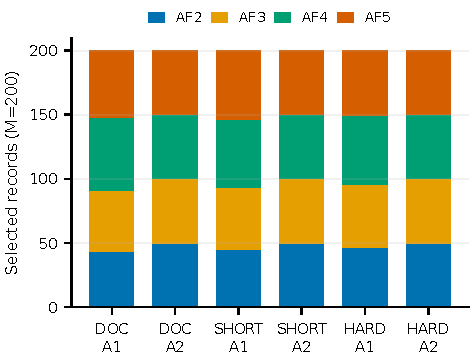
\includegraphics[width=0.43\textwidth]{figures/revision4_stage_memory_composition.pdf}\hfill
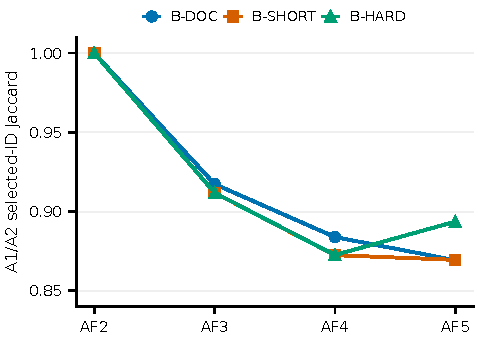
\includegraphics[width=0.43\textwidth]{figures/revision4_selected_buffer_overlap.pdf}
\caption{Controlled memory composition and selected-ID overlap. Class and stage quotas alter selected membership; all methods use canonical replay order. The overlap plot uses a labeled zoomed range.}
\label{fig:memory-audit}
\end{figure*}

\paragraph{Capacity sensitivity.}
A separate three-seed A0-v2/A1 grid at $M\in\{50,200,400\}$ finds no stable advantage on both security axes and no monotonic memory-size optimum; the full matched capacity results are summarized in Table~\ref{tab:r3-capacity}.

The historical A0--A5 sequence remains operational provenance because A1--A3 used separate rank streams. All 36 actual eligible pools have unique coverage keys; under shared ranks, A2 and A3 select identical ordered buffers, leaving the coverage effect untested. The controlled $M=200$ comparison is A0-v2/A1/A2-canonical only. Original Reservoir, CE, and security-risk selectors remain contextual under an earlier numerical protocol. Full historical outcomes remain in the project technical reports.

\begin{figure*}[t]
\centering
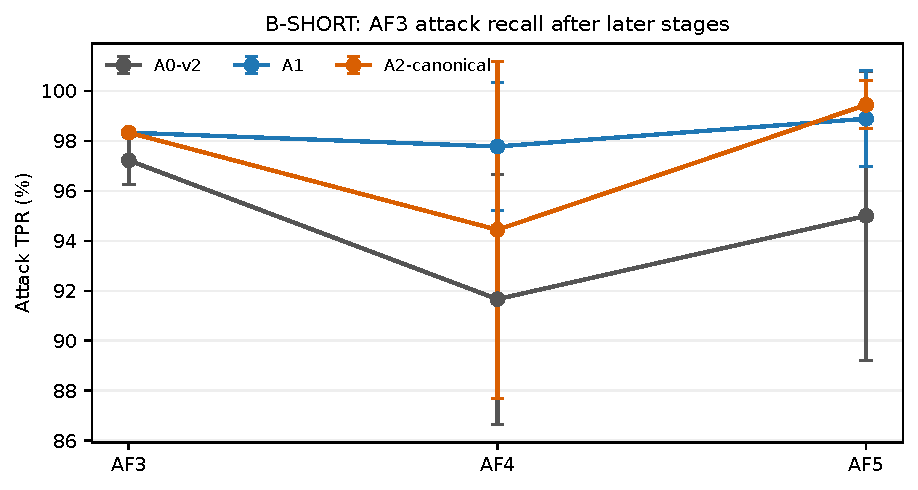
\includegraphics[width=0.48\textwidth]{figures/revision4_b_short_attack_forgetting.pdf}\hfill
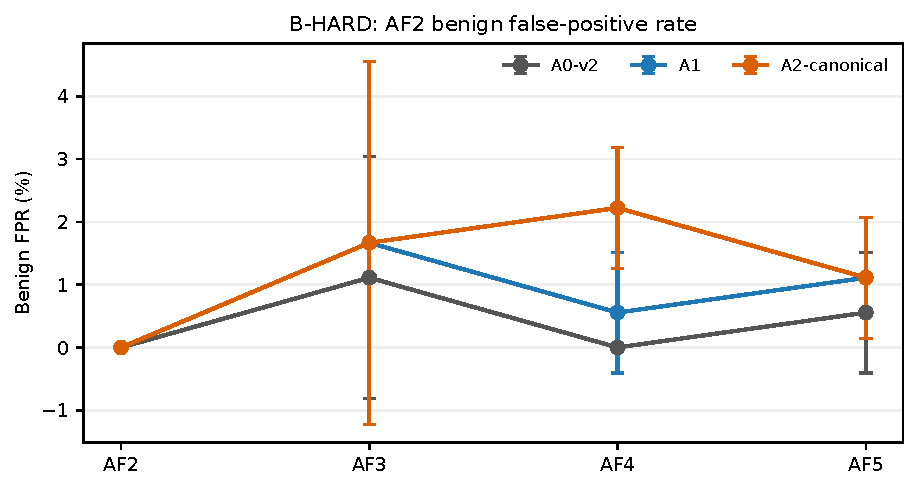
\includegraphics[width=0.48\textwidth]{figures/revision4_b_hard_benign_fpr.pdf}
\caption{Controlled A0-v2/A1/A2-canonical fixed-test trajectories, mean with sample-SD whiskers across three seeds. Left: \bshort{} \af{3} attack recall; right: \bhard{} \af{2} benign FPR. Shared ranks and canonical buffer order permit separate class- and stage-quota comparisons; neither yields a consistent gain.}
\label{fig:route-ablation}
\end{figure*}

\begin{table*}[t]
\caption{Matched capacity grid, mean $\pm$ sample SD over three seeds. Rates are in percentage points; A0-v2/A1 share numerical and replay-index settings. Online Reservoir is excluded.}
\label{tab:r3-capacity}

\centering
\small
\setlength{\tabcolsep}{3pt}
\begin{tabular*}{\textwidth}{@{\extracolsep{\fill}}lllr rrr@{}}
\toprule
Arm & $M$ & Method & TPR BWT & FPR increase & Acq. TPR & Final FPR \\
\midrule
B-SHORT & 50 & A0 & $-0.93\pm1.60$ & $+4.26\pm7.38$ & $99.58\pm0.42$ & $4.03\pm5.90$ \\
B-SHORT & 50 & A1 & $-0.19\pm1.40$ & $+0.56\pm0.56$ & $99.31\pm0.64$ & $1.25\pm0.83$ \\
B-SHORT & 200 & A0 & $-0.56\pm1.47$ & $+0.19\pm0.32$ & $99.17\pm0.42$ & $0.83\pm0.72$ \\
B-SHORT & 200 & A1 & $+0.19\pm0.64$ & $+0.74\pm2.31$ & $99.58\pm0.00$ & $1.25\pm1.44$ \\
B-SHORT & 400 & A0 & $-0.19\pm1.28$ & $-0.19\pm0.32$ & $99.44\pm0.48$ & $0.56\pm0.24$ \\
B-SHORT & 400 & A1 & $+0.56\pm0.56$ & $+0.00\pm0.00$ & $99.44\pm0.48$ & $0.56\pm0.24$ \\
B-HARD & 50 & A0 & $-0.19\pm1.28$ & $+0.74\pm1.28$ & $99.58\pm0.42$ & $1.11\pm0.87$ \\
B-HARD & 50 & A1 & $+0.56\pm0.56$ & $+2.04\pm4.02$ & $99.31\pm0.64$ & $2.36\pm3.37$ \\
B-HARD & 200 & A0 & $+0.37\pm0.32$ & $+0.00\pm0.56$ & $99.31\pm0.24$ & $0.56\pm0.24$ \\
B-HARD & 200 & A1 & $+0.19\pm0.32$ & $+0.19\pm0.32$ & $99.44\pm0.24$ & $0.69\pm0.24$ \\
B-HARD & 400 & A0 & $-0.56\pm2.42$ & $-0.19\pm0.32$ & $99.44\pm0.48$ & $0.42\pm0.00$ \\
B-HARD & 400 & A1 & $-0.56\pm1.92$ & $-0.19\pm0.32$ & $99.44\pm0.48$ & $0.42\pm0.00$ \\
\bottomrule
\end{tabular*}


\end{table*}


\subsection{Acquisition and position diagnostics}

Every method passes 12/12 arm-stage acquisition gates; Table~\ref{tab:acq-summary} reports the worst acquisition observations across all 36 arm--seed--stage cells per method. The minimum attack TPR is 93.333\% for DER++ and at least 95.000\% for every other method. Each method's smallest acquisition macro-F1 remains at least 95.831\%. Thus a large final recall drop is not simply an unlearned stage at first acquisition.

\begin{table}[t]
\caption{Worst acquisition diagnostics (percent) across every arm, stage, and seed. Gate counts here are per-seed cells.}
\label{tab:acq-summary}

\centering
\small
\resizebox{\columnwidth}{!}{%
\begin{tabular}{@{}lrrrr@{}}
\toprule
Method & Min TPR & Max FPR & Min macro-F1 & Gates \\
\midrule
No Replay & 98.333 & 5.000 & 97.498 & 36/36 \\
Reservoir ER & 96.667 & 3.333 & 97.500 & 36/36 \\
DER++ & 93.333 & 3.333 & 95.831 & 36/36 \\
Security-aware & 98.333 & 6.667 & 96.663 & 36/36 \\
Loss-aware & 95.000 & 3.333 & 96.666 & 36/36 \\
\bottomrule
\end{tabular}
}


\end{table}

 Thus, the large No Replay deviations cannot be explained by a general failure to learn later stages. The smallest position-specific attack TPR observed anywhere is 10\% for No Replay on the \bshort{} seed-2026 \af{3}-middle slice after \af{5}. The corresponding minima across all replay runs are 90\% for Reservoir, 85\% for DER++, 90\% for Security-aware, and are near the same range for Loss-aware. Replay repairs a severe hidden position failure rather than merely changing an average.

\subsection{Security-aware versus generic replay}

Security-aware and generic Loss-aware replay both reduce the principal No Replay failures, but their paired differences are small and mixed across the malicious and benign endpoints; neither dominates. Analytically, true-label CE is $-\log(1-r)$ under one binary model state. Precision, ties and subsequently diverged states can produce operational differences, not distinct semantic ranking. A common-checkpoint audit selected the same 200 IDs in the same order for CE and risk; the maximum numerical deviation from $\mathrm{CE}=-\log(1-r)$ was about $6.1\times10^{-6}$.

\subsection{External-bank and source-qualification audit}
The 339-record NotInject bank is sourced from PIGuard, while a separate 120-record B-short bank probes ordinary short-form benign acceptance. These banks did not influence thresholding, epochs, buffer construction, or replay entry. After AF5, B-Doc NotInject FPR ranges across methods from $69.715\pm15.933$ to $92.527\pm4.686$ percentage points; B-short-bank FPR ranges from $37.222\pm7.561$ to $63.333\pm4.640$ points. In B-Short and B-Hard, replay-method NotInject means are between zero and 1.672 points and B-short-bank FPR is zero. Their differing sources and language composition prevent a causal claim about a single benign feature. Replay improves Candidate B retention without fixing B-Doc's severe external over-defense. A model can pass internal balanced tests while remaining unsuitable as a general benign guard.



Independent malicious confirmation was considered but not executed. The earlier family-disjoint and H2-mini streams informed benchmark escalation before Candidate B was frozen and share source material. In a hash-only audit, each earlier TRAIN source contained all 1,600 unique Candidate B TRAIN text hashes, and each earlier TEST source all 480 Candidate B TEST hashes. H2-mini also overlapped normalized and model-view hashes, native IDs, and source parents; renaming these records would not create independent replication. Public BIPIA, InjecAgent, AgentDojo, AgentDyn, and WAInjectBench candidates lacked at least one verified requirement among usable terms, a fixed binary detector view, parent-disjoint splits, duplicate and semantic-neighbor controls, and prospective ordered stages. WAInjectBench's published 991 malicious and 2,707 benign text segments are not a qualified sequence for this experiment \cite{liu2026wainjectbench}. We report the eligibility audit, not a negative replication result.
\subsection{Interpretation and independent validation}
Continual security evaluation must preserve both error directions: a detector can remember attacks but reject benign content, or accept benign content while forgetting an attack. Strong acquisition in \candb{} locates its large failures in retention. Earlier family and H2-mini streams saturated; the prospective R0/R1/R2 policy delayed replay until the more demanding \candb{} stream was frozen. Its document-to-short and hard-benign transitions coincide with attack and benign-boundary changes, respectively, but source, format, language, length, and semantics are not isolated.

All replay methods reduce the principal No Replay deviations on \candb{}. Re-exposure to retained historical malicious and benign records plausibly contributes: extra current-only exposure remains behind Reservoir, yet different historical access prevents a pure computation or mechanism attribution. Reservoir remains competitive; DER++ has no decisive advantage at this budget. Balanced class proportions may limit the marginal class-quota effect. Stage quotas bind in 27/36 pools, but the controlled selectors give mixed small TPR/FPR effects. Coverage never binds; risk and CE have the same common-state ranking. These findings do not prove selector equivalence.

No independent confirmation was executed. Previously explored streams overlap \candb{}; the public IPI candidates audited in our source audit lack the requisite rights, binary-view, parent/near-neighbor and prospective-stage checks. This is an eligibility result, not a negative replication. Efficacy conclusions remain \candb{}-specific.

\section{Conclusion and Future Work}
On Candidate B, current-only sequential updates caused seed-variable malicious forgetting and benign over-defense despite strong stage acquisition. At a 200-example memory, four replay methods reduced the principal failures. Additional current-only exposure did not reach their endpoints; simple Reservoir ER remained competitive. A matched selector ablation found no stable security gain from class or historical-stage quotas, despite changed memory memberships. These results favor evaluating both directions of error and including a simple replay baseline before claiming the need for a specialized selector.

The conclusions are narrow. We tested one detector revision, one four-stage order, three seeds, finite balanced test sets, and a constructed stream; AF5 combines earlier components rather than representing a new disjoint family. The arms bundle source, format, language, length, and semantics, so observed differences cannot be causally assigned to a single factor. The additional-current-data control differs from replay in information access and therefore cannot isolate computation. The CE/risk equivalence concerns one common model state; later selected memories and model states can diverge. The coverage rule never binds on actual pools, leaving its effect untested. External benign banks are diagnostic, not matched deployment tests.

Future work should qualify an independently sourced IPI stream with usage-rights, parent-disjoint splits, a fixed binary detector view, near-neighbor checks, and prospective stage order before training; the currently audited public candidates have not passed all these gates. Further studies should vary detector architecture, order, memory capacity, and replay exposure, and test live retrieval settings and adaptive attacks. Larger independent samples are needed to estimate whether the small quota effects are meaningful. Until such studies, this report does not establish deployment readiness or a universal replay advantage.

\section*{Author Contributions}
Haoxiang Liao led study design and analysis. Leshan Tang led experimentation and writing.

\clearpage
\bibliographystyle{IEEEtran}
\bibliography{references}
\end{document}
